\chapter{Desarrollo de IPFShare}\label{chap:4desarrollo}
Se ha denominado IPFShare al sistema de intercambio de archivos desarrollado en este proyecto.
\section{Requisitos y definición del sistema}
En esta sección se definen los requisitos funcionales y no funcionales que debe integrar el sistema propuesto.
\subsection{Requisitos funcionales}
\begin{itemize}[noitemsep,after=\vspace{-0.6\baselineskip}]
  \item Un usuario debe poder autenticarse en el sistema.
  \item Un usuario debe poder compartir archivos y directorios con uno o varios usuarios.
  \item Un usuario debe poder descargar archivos y directorios compartidos por otros usuarios del sistema.
  \item A la hora de compartir un archivo un usuario debe poder elegir con qué otros usuarios del sistema compartirlo.
  \item Un usuario debe tener posibilidad de hacer grupos de compartición.
  \item Cuando un usuario comparta recursos con otros usuarios, estos deben recibir una notificación.
  \item Un usuario debe poder interactuar las comparticiones que ha realizado.
  \item Un usuario debe poder interactuar las comparticiones que le han realizado.
\end{itemize}
\subsection{Requisitos no funcionales}
\begin{itemize}[noitemsep,after=\vspace{-0.4\baselineskip}]
  \item El sistema debe proporcionar una interfaz de usuario intuitiva y fácil de usar.
  \item El sistema debe implementar servicios de seguridad en torno a la autenticación.
  \item El sistema debe proporcionar medidas de seguridad para los archivos compartidos.
  \item El sistema debe proporcionar un servicio o mecanismos de identificación de usuario portable.
  \item Las transacciones y eventos del sistema deben ser relativamente instantáneos.
\end{itemize}
Hay que destacar que este sistema no propone la sincronización de archivos que normalmente se asocia con los sistemas de
almacenamiento en la nube. Incluir el desarrollo de esta funcionalidad en el sistema propuesto no es algo trivial.
La sincronización de datos en tiempo real es un tópico muy complejo y se sale
del alcance de este proyecto. Sin embargo, en la sección de \nameref{chap:7trabajosfuturos} dentro de las posibles
mejoras se propone una posible implementación de esta funcionalidad.
\section{Arquitectura y diseño}

Uno de los objetivos de este trabajo es comparar la viabilidad de IPFS como alternativa a los sistemas centralizados.
En esta sección se presenta una arquitectura simplificada para un sistema de intercambio de archivos centralizado habitual.
Después se contrastará con la alternativa descentralizada propuesta.

\subsection{Arquitectura de un sistema de intercambio de archivos centralizado habitual}

Como se puede observar en la figura \ref{fig:centralizedarch}, la arquitectura de un sistema de intercambio de archivos
requiere de varios puntos de acceso centralizados para funcionar\footnote{Este diseño se ha ideado tomando como referencia los siguientes recursos:
  \cite{chakrabortySystemDesignAnalysis2020} y
  \cite{systemdesignSystemDesignInterview2023}.}.En un caso real esta arquitectura podría ser más compleja, implementando sistemas de caching, entre otras muchas mejoras posibles. Para este ejemplo se ha simplificado para centrarse en los puntos clave.

Existe una clara separación conceptual de las distintos componentes, aunque pueden estar ubicados en
el mismo servidor físico, en varios, o incluso, cada servicio en varios servidores físicos. Esto depende de la escala
del sistema y de las necesidades de rendimiento y disponibilidad.

\begin{itemize}[noitemsep,after=\vspace{-0.4\baselineskip}]
  \item \textbf{Almacenamiento cloud:} el almacén donde se guardarán los chunks de ficheros proporcionados por el servicio
        de procesamiento de ficheros, Amazon S3 es un ejemplo de un servicio de estas característica.
        \item\textbf{Servicio de procesamiento de ficheros:} es el encargado atender y llevar a cabo las peticiones de usuario relacionadas con ficheros.
  \item \textbf{Servicio de autenticación:} gestiona la autenticación de los usuarios. Contiene los datos de los usuarios y sus credenciales.
  \item \textbf{Servicio de metadatos:} se encarga de enviar las notificaciones de los usuarios. Cuando un cliente
        comparte un fichero con otro, el cliente envía también una serie de metadatos sobre esta acción que acaba de realizar.
        Estos metadatos se pueden usar para gran variedad de propósitos. En este caso se usan para implementar un servicio de notificaciones basado en colas de mensajes.
\end{itemize}
\begin{sidewaysfigure}
  \centering
  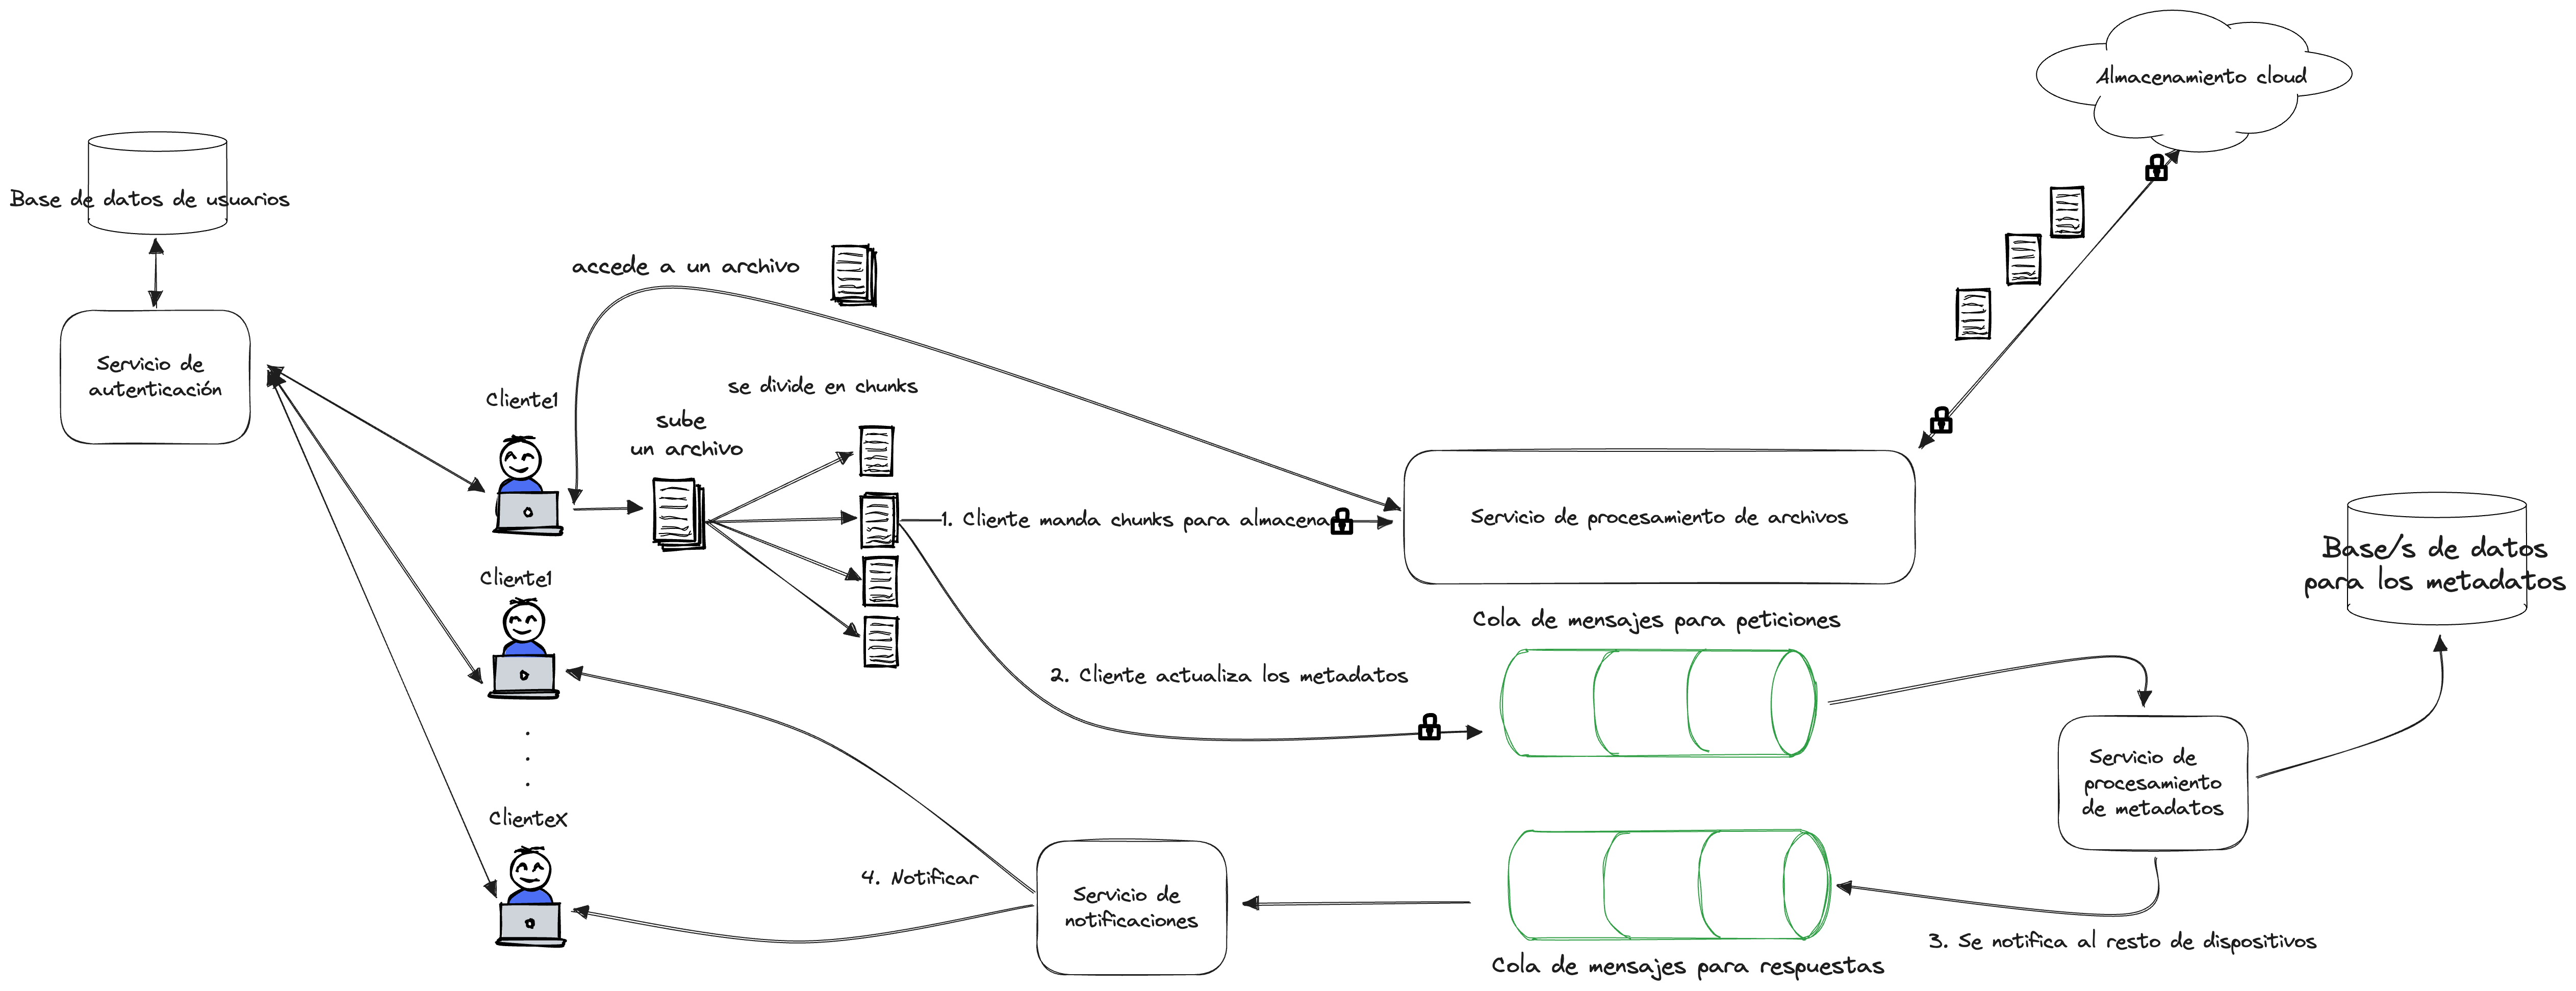
\includegraphics[width=\textwidth]{images/diagramacentral.png}
  \caption{Posible arquitectura de un servicio centralizado de archivos}
  \label{fig:centralizedarch}
\end{sidewaysfigure}

Cuando un cliente quiere compartir un fichero, este divide el archivo en trozos más pequeños llamados chunks\footnote{En un servicio de compartición de archivos, los archivos se subdividen en fragmentos o chunks para mejorar la eficiencia de la transferencia de datos, permitiendo la transmisión paralela y la reanudación de las transferencias interrumpidas, así como facilitar la distribución del almacenamiento y reducir la redundancia de datos.}.
Envía a través de una conexión segura (socket tpc sobre TLS por ejemplo) estos chunks que componen el archivo al servicio de procesamiento de ficheros.
Este servicio se encarga de guardar los chunks en el almacenamiento cloud y de mandar los metadatos a la cola de mensajes.
El servicio de metadatos procesa de forma asíncrona estos metadatos, extrayendo la información pertinente que identifique
a los usuarios y el recurso compartido. Después envía una notificación a los usuarios que corresponda.

Dado que el servicio de autenticación posee datos de los usuarios, cuando un usuario quiera enviar un archivo puede
pedir esta al servicio de autenticación, el incluso se podría combinar con el servicio de metadatos para brindar otras funcionalidades como ver los recursos que se le han compartido o los usuarios con los que se ha compartido.

Bajo este sistema los clientes deben saber de antemano dónde se ubican estos servicios para poder interactuar con
ellos. Estos servicios podrían ser provistos por entidades externas (lo cual es muy habitual en un sistema de este estilo), creando dependencias en
sistemas centralizados de terceros.
\subsection{Arquitectura de IPFShare: un sistema de intercambio de archivos descentralizado}
En comparación con la arquitectura anterior (figura \ref{fig:centralizedarch}), la arquitectura de IPFShare es
completamente descentralizada. No existe ningún servicio centralizado, cualquier servicio proporcionado por una entidad externa proviene de
de otros nodos IPFS, siendo el propio nodo cliente otro proveedor más de servicios. Esto hace el sistema completamente autocontenido e independiente de servicios fuera
de la red IPFS.

\begin{figure}[H]
  \centering
  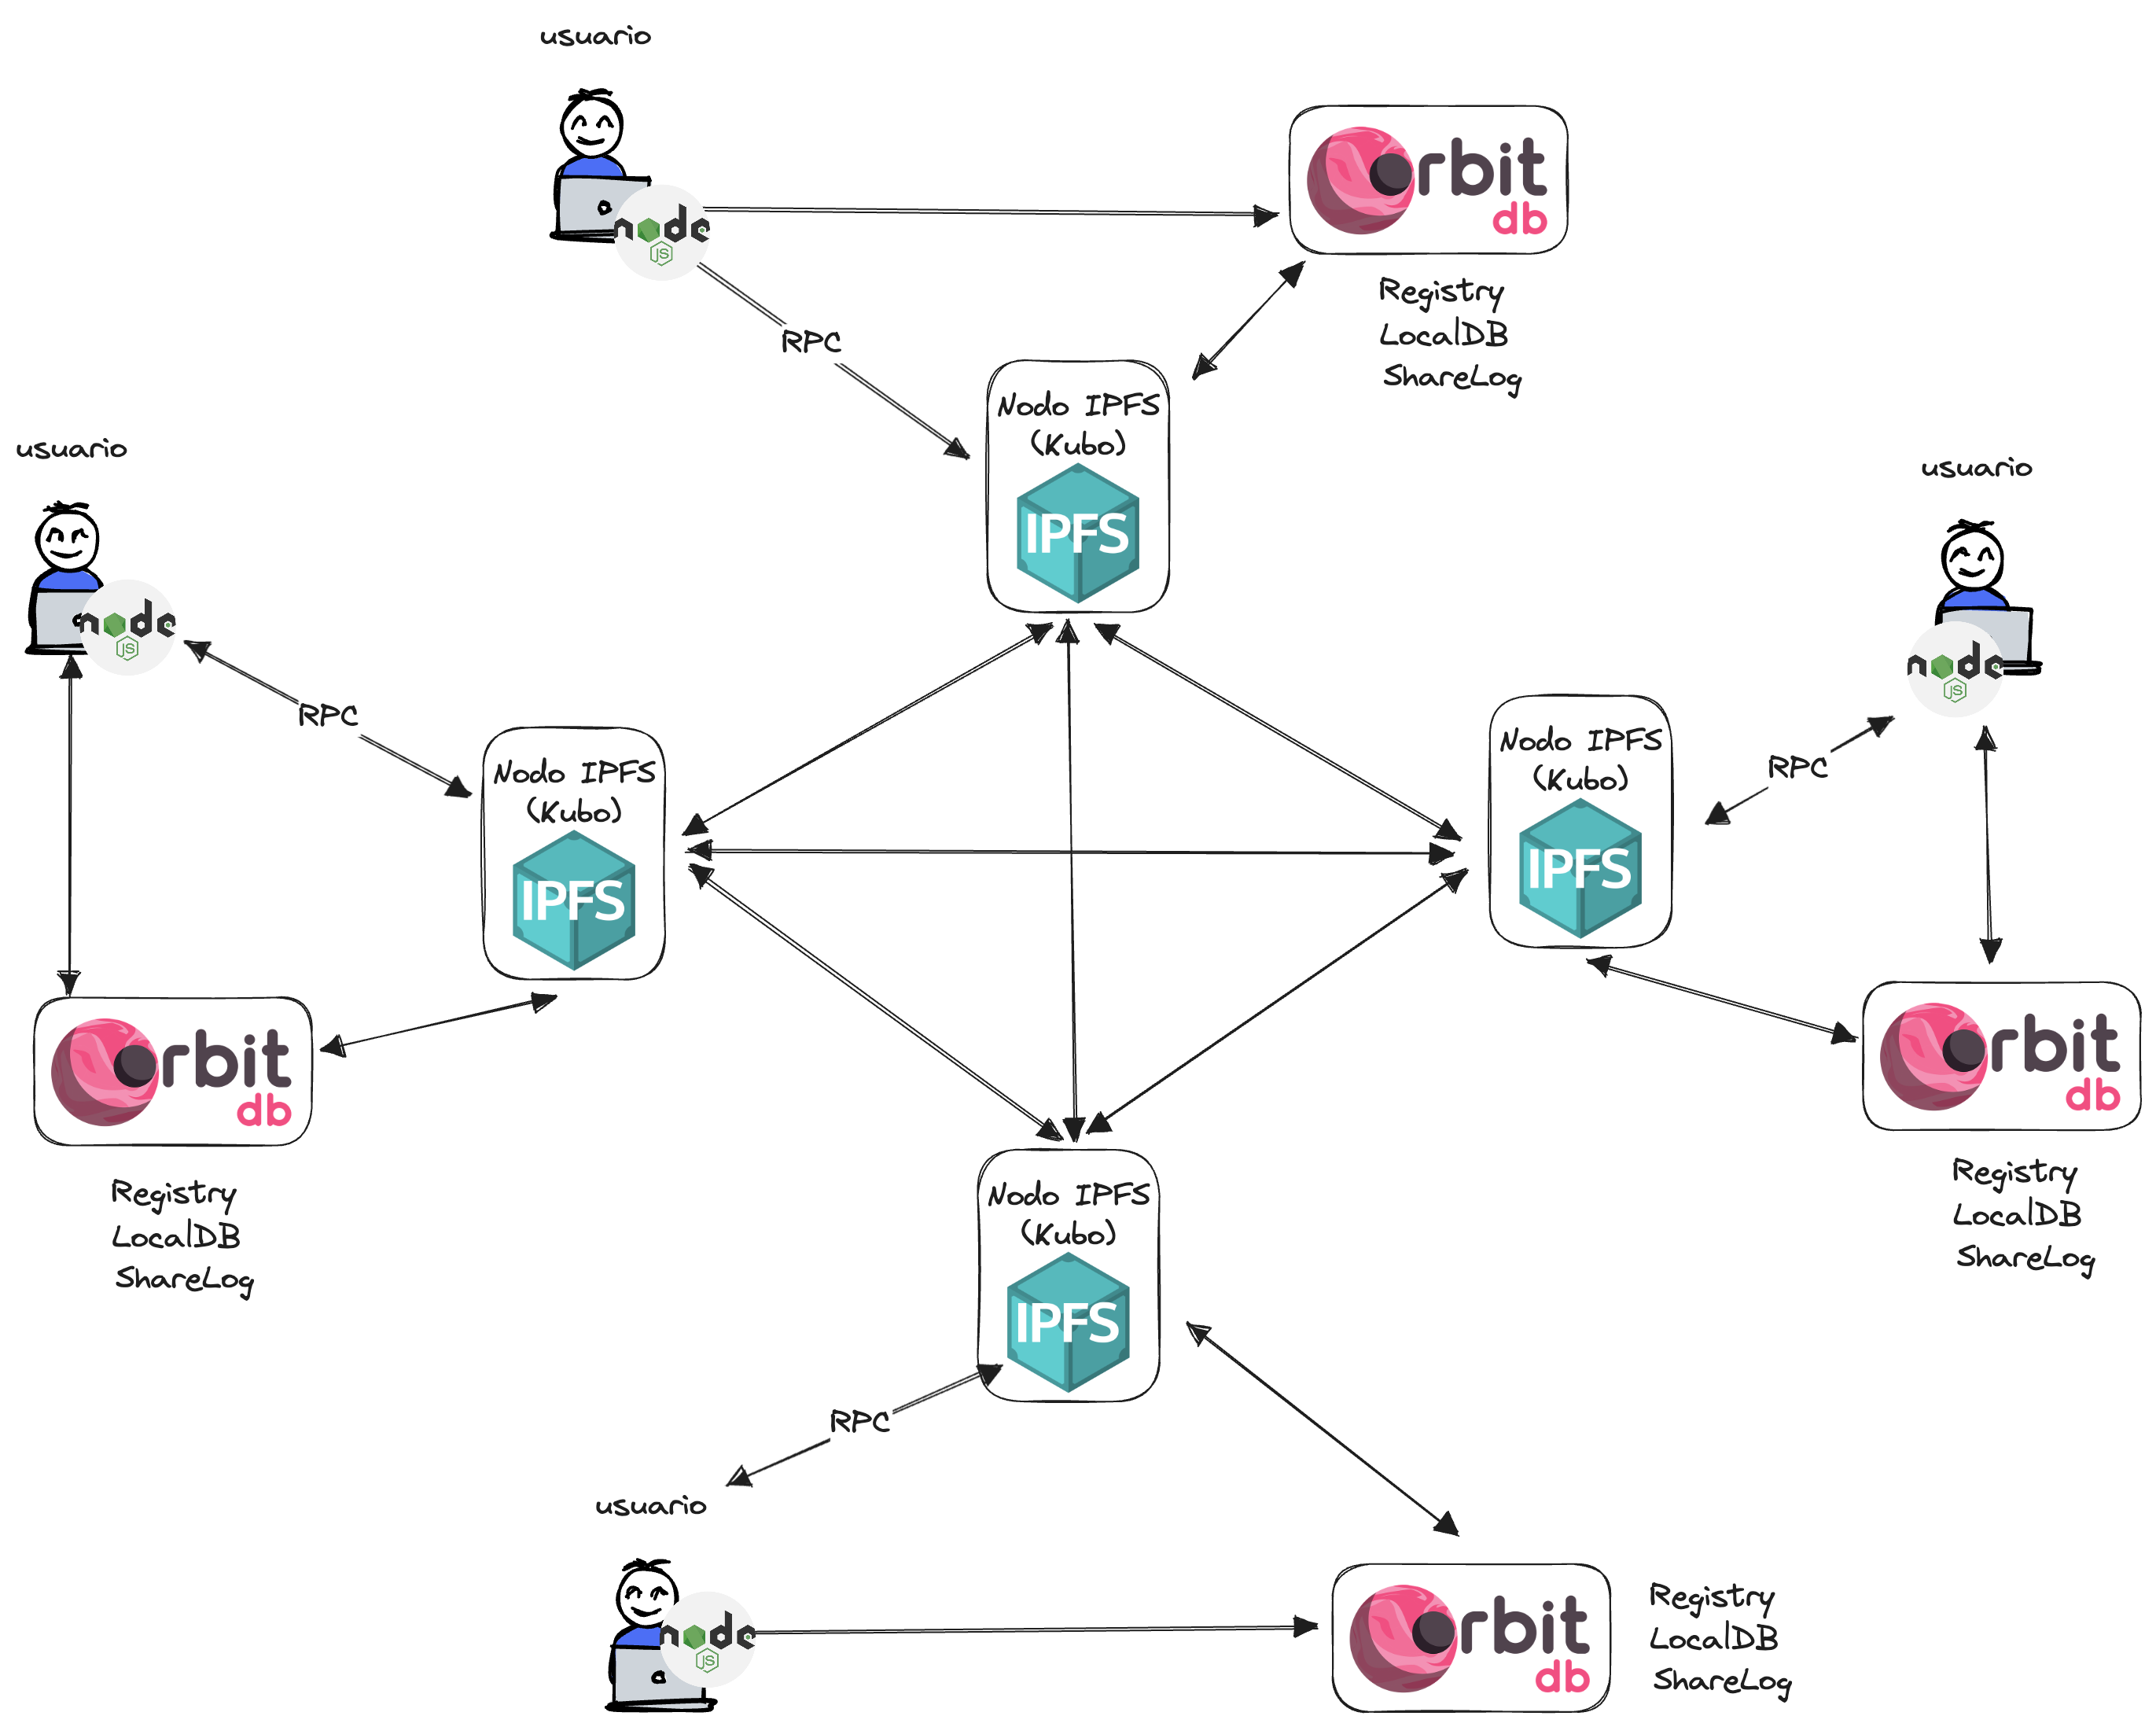
\includegraphics[width=\textwidth]{images/ipfshare-architecture.png}
  \caption{Arquitectura de IPFShare}
  \label{fig:ipfsharearch}
\end{figure}

En el sistema propuesto, cada usuario opera un nodo IPFS, que sirve como su punto de conexión a la red IPFS. Las interacciones entre el cliente y
este nodo IPFS se facilitan a través de una interfaz de programación de aplicaciones (API), que expone un conjunto de operaciones que puede realizar
el nodo \cite{KuboRPCAPI}. Esta comunicación se lleva a cabo mediante RPC, un protocolo que permite al cliente ejecutar procedimientos en el nodo IPFS como si estuvieran en el mismo sistema, lo que facilita la solicitud eficiente de servicios y operaciones.

El programa interactúa con la red IPFS mediante esta API a través del nodo IPFS local. IPFS sustituye al servicio de almacenamiento cloud
al ser un gran swarm de nodos que almacenan y comparten datos entre sí. IPFS en sí mismo no impone un límite teórico sobre la cantidad de datos que
pueden ser subidos a un nodo que se comporta correctamente. El límite práctico vendría determinado por factores como los recursos del sistema (espacio en
disco, ancho de banda de red, etc.), la configuración del nodo IPFS y cualquier restricción impuesta por la red o el proveedor de alojamiento. Proveedor
de alojamiento quiere decir otros nodos IPFS que compartan el mismo (o parte del) pinset que el nodo del usuario.

El servicio de procesamiento de ficheros se sustituye también por IPFS. El proceso de añadir cualquier dato a IPFS implica la subdivisión en chunks
para la generación del DAG y el uso de este en Bitswap, como ya se explicó en el apartado \ref{sect:modelo-de-datos}: '\nameref{sect:modelo-de-datos}'.

El servicio de autenticación se sustituye por un sistema de identificación descentralizado basado en DIDs que opera mediante
lo que se ha denominado como un \textit{Registry}. Un Registry es una base de datos distribuida que almacena información sobre los usuarios del sistema.
Esta base de datos distribuida es provista por OrbitDB, del cual se hablará más tarde en el apartado \ref{sect:tecnologias}.

El concepto principal consiste
en que cada cliente tiene un instancia de OrbitDB que opera mediante IPFS. Esta instancia de OrbitDB mantiene constancia de una serie de bases de datos distribuidas que se sincronizan
con el resto de nodos, intercambiando los datos que se han modificado o añadido. De esta forma, se consigue una base de datos replicada y consistente entre todos los participantes del
sistema. OrbitDB ofrece diferentes tipos de bases de datos, como colecciones de documentos, claves-valor o registros de eventos. Para el caso del Registry, se utiliza una base de
datos de tipo clave-valor, donde la clave es el DID del usuario y el valor es un objeto JSON que contiene el peerID del usuario, su DID y un alias.
\begin{itemize}[noitemsep,after=\vspace{-0.4\baselineskip}]
  \item El DID es un identificador único que se genera a partir de la clave privada del usuario.
        Se utiliza como identidad de la instancia de OrbitDB para permitir verificar la autoría de las entradas en el registro.
  \item El alias es un nombre que el usuario puede elegir para identificarse en el sistema. Puede hacerse único o no, dependiendo de la política de acceso del Registry.
\end{itemize}

Un Registry debe incorporar un controlador de acceso que mantiene una serie de políticas de acceso respecto del mismo.
Estas políticas son:
\begin{itemize}[noitemsep,after=\vspace{-0.4\baselineskip}]
  \item Cualquier usuario puede crear una entrada en el registro.
  \item Un usuario solo puede tener una entrada en el registro.
  \item Solo el usuario que creó la entrada una puede modificarla.
  \item Solo el usuario que creó la entrada una puede eliminarla.
\end{itemize}


Cuando se crea una instancia de OrbitDB, el creador especifica un controlador de acceso (AC) para la base de datos.
Este controlador de acceso se almacena en el manifiesto de la base de datos (los metadatos de la base de datos)
y la dirección de este manifiesto se utiliza luego para cargar la base de datos. Entonces surge la pregunta, ¿no podría alguien simplemente intercambiar el controlador de acceso en su instancia local?
\\
La respuesta a esto es no, no pueden por las siguiente razones:
\begin{enumerate}[noitemsep,after=\vspace{-0.4\baselineskip}]
  \item El controlador de acceso y sus parámetros se almacenan en el manifiesto de la base de datos, y el hash de este manifiesto compone la dirección de la base de datos. Si alguien cambia el controlador de acceso, cambiarían el manifiesto, y por lo tanto la dirección de la base de datos. Esencialmente, estarían creando una base de datos completamente nueva, no alterando la original.
  \item Incluso si alguien crea una nueva base de datos con un controlador de acceso diferente, no pueden escribir en la base de datos original al no concordar las direcciones.
  \item Todas las actualizaciones a la base de datos (adiciones, modificaciones, etc.) son firmadas por las claves privadas del escritor. Si un usuario malintencionado intenta alterar los datos, las firmas no coincidirán, haciendo que los cambios sean invalidados por el resto de nodos que poseen la base datos.
  \item Al leer de la base de datos, el controlador de acceso valida si los datos (entradas) pueden ser añadidos a la base de datos local o no. Incluso si alguien cambiara el controlador de acceso localmente, no podrían alimentar datos alterados a otros porque los controladores de acceso de los demás validarían y rechazarían los cambios.
\end{enumerate}

Este sistema de control de acceso basado en estructuras de datos inmutables, firmas y consenso es lo que hace que OrbitDB sea una base de datos distribuida segura y confiable.




\section{Tecnologías usadas}\label{sect:tecnologias}


\section{Implementación}


\begin{minted}{typescript}
import OrbitDB from "orbit-db"
// eslint-disable-next-line @typescript-eslint/ban-ts-comment
// @ts-ignore
import AccessController from "orbit-db-access-controllers/interface"
import DocumentStore from "orbit-db-docstore"
import { IdentityProvider } from "orbit-db-identity-provider"

export interface RegistryEntry {
    peerId: string
    orbitdbIdentity: string // DID
    username: string // alias
  }

export abstract class Registry<S, DocType> {
    abstract accessController: AccessController
    abstract store: S
    abstract open(): Promise<void>
    abstract create(): Promise<void>
    abstract replicate(): Promise<void>
    abstract close(): Promise<void>
    abstract addUser(user: DocType): Promise<void>
    abstract getUser(entryId: string): Promise<DocType | undefined>
    abstract updateUser(entryId: string, updates: Partial<DocType>): Promise<void>
    abstract searchUsers(queryFn: (entry: DocType) => boolean): Promise<DocType[]>
    abstract deleteUser(entryId: string): Promise<void>
  }
\end{minted}